
\documentclass[14pt,a4paper]{extarticle}
\usepackage[utf8]{inputenc}
\usepackage[T1]{fontenc}
\usepackage[french, provide=*]{babel}
\usepackage{graphicx}
\usepackage{geometry}
\geometry{a4paper, margin=2.5cm}
\usepackage{hyperref}
\usepackage{fancyhdr}
\usepackage{titlesec}
\usepackage{enumitem}
\usepackage{booktabs}
\usepackage{xcolor}
\usepackage{tabularx}
\usepackage{float}
\usepackage{setspace}
\usepackage{pdfpages}



\setstretch{1.2}

\hypersetup{
    colorlinks=true,
    linkcolor=blue!70!black,
    urlcolor=blue!70!black,
    citecolor=blue!70!black
}

\pagestyle{fancy}
\fancyhf{}
\fancyhead[L]{\textbf{Projet Développement Web 2}}
\fancyhead[R]{Rapport de Projet}
\fancyfoot[C]{\thepage}
\renewcommand{\headrulewidth}{0.5pt}
\renewcommand{\footrulewidth}{0.5pt}

\title{
    \vspace*{4cm}
    \rule{\linewidth}{1mm} \\[0.5cm]
    \Huge{\textbf{Rapport de Projet}} \\
    \vspace{0.5cm}
    \Large{Développement Web 2 - L3 Informatique} \\
    \vspace{0.5cm}
    \textbf{Éditeur de texte collaboratif en temps réel}
    \rule{\linewidth}{1mm} \\[4cm]
}
\author{
    	\textbf{GIRAUD NICOLAS} \\
    	\textbf{COURT ANTHONY} \\
    	\textbf{CONTANT THIBAULT}
}
\date{\vspace*{2cm} \today}

\begin{document}

\maketitle
\thispagestyle{empty}
\newpage

\tableofcontents
\thispagestyle{empty}
\newpage

\setcounter{page}{1}

\section{Introduction}
\label{sec:intro}
Dans le cadre de l'enseignement "Développement Web 2" du semestre 6, nous avons choisi de concevoir une application web interactive.

Notre choix s'est porté sur la réalisation d'un \textbf{éditeur de texte collaboratif en temps réel}. Cette application permet à plusieurs utilisateurs de se connecter, de créer des documents, de gérer des droits d'accès avancés (propriétaire, éditeur, lecteur) et de modifier simultanément un même fichier tout en communiquant via une messagerie instantanée intégrée. 

Ce rapport présente en détail la conception de notre application.

\section{Description de l'application et fonctionnalités}
\label{sec:fonctionnalites}

L’application que nous avons développée est un environnement d'édition de texte collaboratif en ligne Son objectif principal est de permettre à plusieurs utilisateurs de gérer et d'éditer des documents de manière sécurisée et interactive. Notre application propose une gestion des droits d'accès et permet une communication en temps réel grace à l'utilisation des WebSockets.

\subsection{Gestion des utilisateurs et authentification}
Lorsque l'on arrive sur la page d'accueil du site, les utilisateurs doivent s'inscrire puis se connecter pour accéder à la plateforme. Les administrateurs  du site disposent de privilèges supérieurs dès leur connexion, leur permettant de modérer la plateforme en ayant la possibilité de supprimer des utilisateurs ou des documents.

\subsection{Gestion des documents et des droits d'accès}
Une fois authentifié, l'utilisateur accède au tableau de bord principal (la page DocumentChoice). L'application permet d'y créer un nouveau document – ce qui génère automatiquement un fichier sur le serveur – ou d'en rechercher un existant. LChaque document est régi par une table de permissions stricte offrant trois niveaux d'implication :

    \begin{description}
    \item[\textbf{OWNER (Propriétaire) :}] Ce rôle est attribué par défaut au créateur du document. Le propriétaire détient les droits absolus sur son fichier. Il peut l'éditer, inviter d'autres utilisateurs en leur octroyant des droits d'écriture, bannir des lecteurs, ou encore supprimer définitivement le document du serveur.
    
    \item[\textbf{WRITER (Éditeur) :}] Les utilisateurs invités avec ce rôle peuvent participer activement à la rédaction. Ils ont la capacité de modifier le document, de sauvegarder leurs modifications sur le serveur et de télécharger le fichier sur leur propre machine.
    
    \item[\textbf{VIEWER (Lecteur) :}] Par défaut, le reste des membres du site se voit attribuer ce rôle sur un nouveau document public. Ils peuvent uniquement consulter le contenu sans avoir la possibilité de le modifier.
\end{description}

\subsection{Édition collaborative et communication}
Enfin, l'espace de travail (Editor) constitue le cœur  du projet. Cette interface affiche la liste des collaborateurs ayant accès au document en cours et précise leur rôle. L'édition du texte est rendue dynamique grâce aux WebSockets qui permettent de gérer les modifications en temps réel. Nous avons aussi intégré un système de messagerie instantanée (Chat) permettant aux utilisateurs d'échanger en direct pendant qu'ils travaillent sur un même document.

\section{Conception et Architecture}
\label{sec:conception}

\subsection{Diagramme UML}
Voici le diagramme UML de notre projet \\
Ce diagramme a été réalisé grâce a UMLet
\begin{figure}[H]
    \centering
    % [page=1] permet de choisir la page du PDF à afficher
    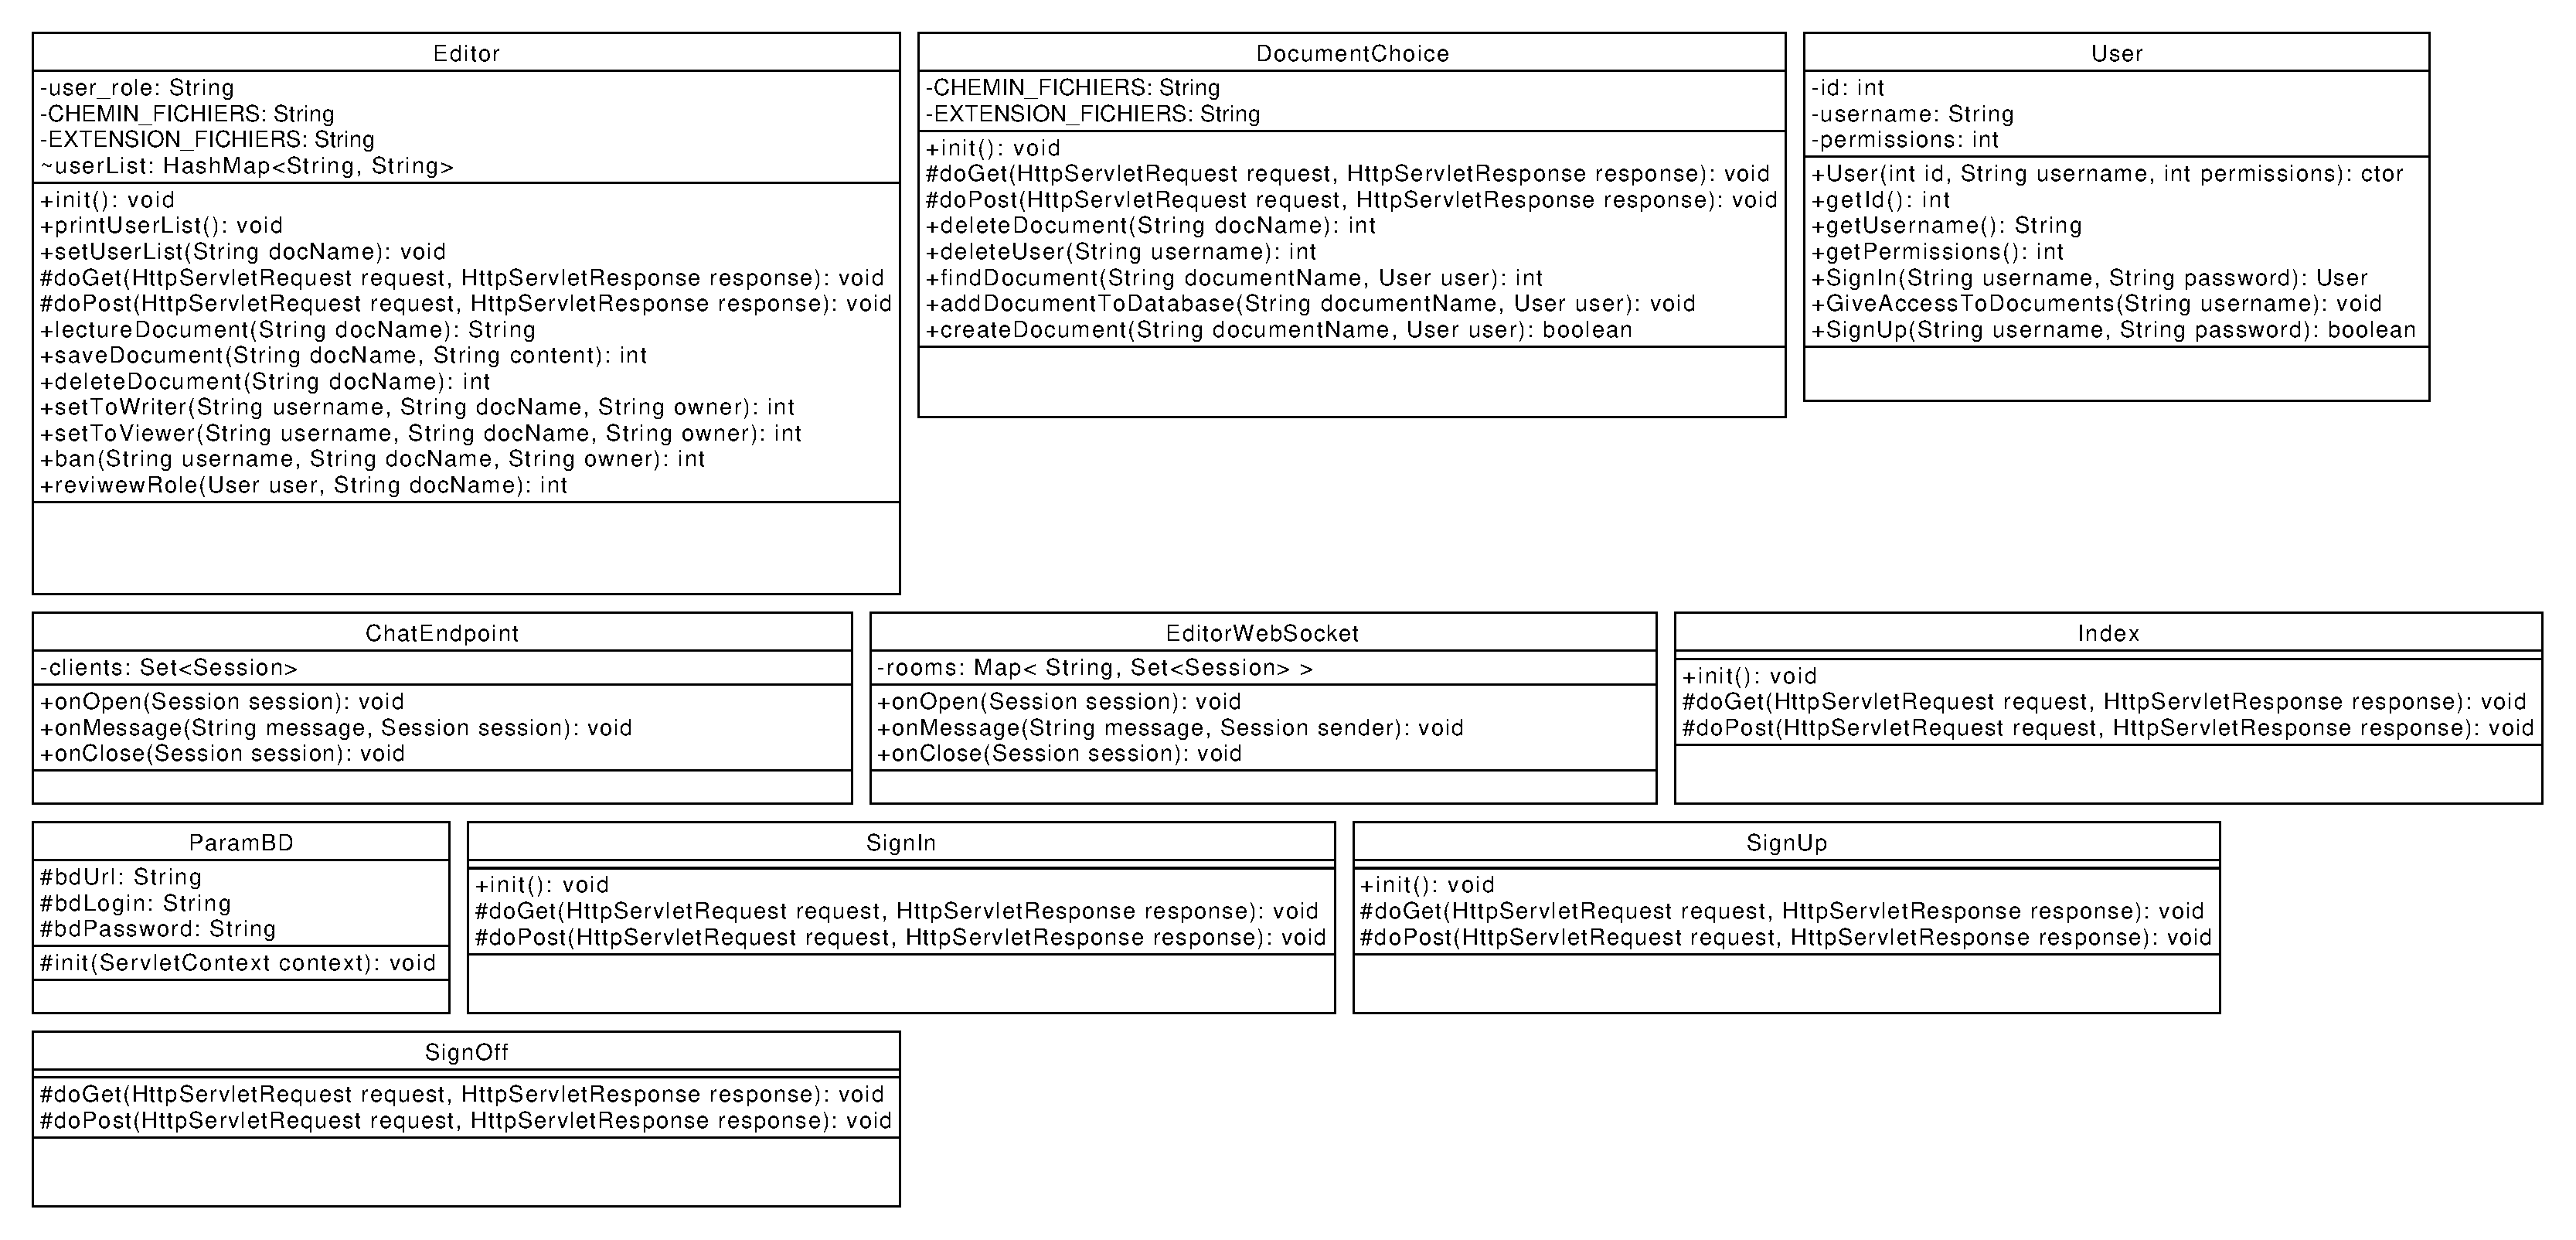
\includegraphics[width=0.95\linewidth, page=1]{UML_Projet_Web.pdf}
    \caption{Diagrammes UML du projet - Page 1}
\end{figure}
Notre application possède plusieurs grandes fonctionnalités : 
D'abord, la gestion des utilisateurs : les classes SignIn, SignUp et SignOff gèrent la connexion, l'inscription et la déconnexion, en s'appuyant sur la classe User qui stocke les informations de chaque utilisateur (identifiant, nom, niveau de permission).

Ensuite, la gestion des documents : la classe DocumentChoice permet de créer, supprimer et rechercher des documents, tandis que la classe Editor se charge de leur lecture, sauvegarde et modification. L'éditeur gère également les droits d'accès, en permettant d'attribuer à un utilisateur un rôle de lecteur ou de rédacteur, voire de le bannir d'un document.

Enfin, la communication en temps réel est assurée par deux composants WebSocket. EditorWebSocket synchronise les modifications entre les utilisateurs travaillant simultanément sur un même document, et ChatEndpoint propose un système de messagerie intégré.

La classe ParamBD, quant à elle, centralise la configuration de la base de données utilisée par l'ensemble de l'application.



\subsection{Modèle Relationnel}
\begin{figure}[H]
    \centering
    % width=0.8\linewidth permet d'ajuster l'image à 80% de la largeur du texte
    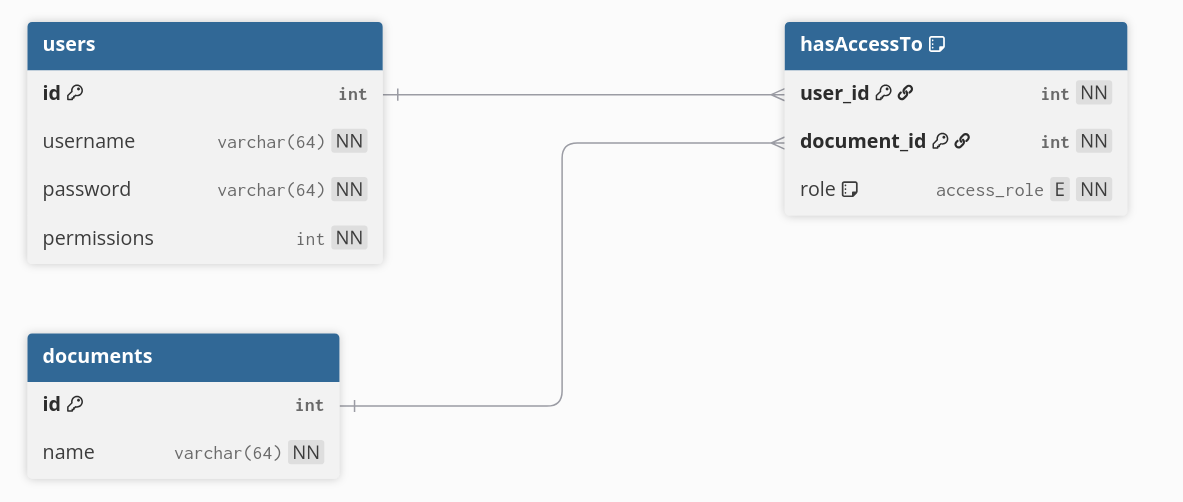
\includegraphics[width=0.8\linewidth]{modele_relationnel.png}
    \caption{Diagramme Relationnel de la Base de Données (users, documents, hasAccessTo)}
    \label{fig:mod_relationnel}
\end{figure}
Notre base de données s'articule autour de trois entités principales. Les tables users et documents sont indépendantes et possèdent chacune un identifiant(clé primaire).
La dernière table "hasAccesTo" permet de lien un utilisateur a un document. Cette table possède un attribut role (défini par une énumération), qui détermine le niveau de privilège de l'utilisateur sur le document.


\section{Bilan des implémentations}
\subsection{Points forts}
\label{sec:realisation}

Nous avons réussi à développer les fonctionnalités principales de notre application. L'inscription et la connexion des utilisateurs fonctionnent parfaitement et sont sécurisées. La création de documents et leur enregistrement dans la base de données sont également opérationnels. Nous avons aussi ajouté un système de role : l'application différencie très bien les Propriétaires, les Éditeurs et les Lecteurs, et donne les bonnes permissions à chacun. Enfin, les administrateurs disposent bien des outils nécessaires pour supprimer des utilisateurs ou des documents en cas de besoin.

\subsection{Limites et points d'améliorations}
\textbf{Le design de l'application (CSS)} : L'interface est restée très basique et visuellement simple. On n'utilise pas JavaScript pour améliorer le design. Nous avons préféré passer notre temps à faire fonctionner la logique du site en arrière-plan plutôt qu'à décorer les pages. \\
\textbf{Présence et Curseurs en temps réel}
L'éditeur ne permet pas de voir où les autres travaillent précisément. Nous aurions pu rajouter des curseurs à l'image de Google Docs, cela éviterait que deux personnes n'essaient de modifier la même phrase en même temps.

\section{Ressources Extérieures Utilisées}
\label{sec:ressources}

Pour mener à bien ce projet, nous avons utilisés  plusieurs outils et bibliothèques externes. Lors de la phase de conception, nous avons eu recours à UMLet pour réaliser notre diagramme UML, tandis que nous avons utilisé la plateforme en ligne dbdiagram.io pour concevoir notre modèle relationnel de base de données. Côté implémentation, notre architecture repose sur le pilote JDBC, placé dans notre dossier WEB-INF/lib. Pour la partie interface utilisateur, nous avons intégré la bibliothèque JSTL (Jakarta Standard Tag Library) à nos vues (.jsp). Cela nous a permis de respecter de respecter les normes de MVC en évitant de mélanger la logique métier et la vue. Le projet s'exécute au sein du serveur d'application Apache Tomcat et utilise les WebSockets  pour assurer la communication en temps réel de l'éditeur et du chat.
\section{Organisation du Travail}
\label{sec:organisation}

Nous avons tenté de répartir le travail de manière équitable. \\
Voici la répartition dans un tableau. \\
Nous avons passé environ 20h chacun sur ce projet \\

\begin{table}[H]
\centering
\begin{tabularx}{\textwidth}{>{\hsize=0.6\hsize}X >{\hsize=1.4\hsize}X >{\hsize=0.15\hsize}c}
\toprule
\textbf{Membre} & \textbf{Rôles et Tâches principales} & \textbf{Temps (est.)} \\ \midrule
\textbf{Nicolas Giraud} & Développement intégral du module de discussion / Création du point d'accès serveur (ChatEndpoint.java) avec l'API WebSockets, et gestion de la connexion asynchrone côté client (chat.js) / Développement du serveur WebSocket pour l'éditeur (EditorWebSocket.java) / Développement de la Servlet DocumentChoice.java gérant la création de documents sur le serveur &\textasciitilde 20h \\ \addlinespace
\textbf{Anthony Court} & Développement complet des Servlets d'inscription (SignUp.java) et de connexion (SignIn.java) / Création des scripts SQL (creation.sql, insertion.sql), définition du modèle relationnel (les 3 tables dont hasAccessTo) et mise en place de la connexion JDBC via la classe ParamBD.java / Intégration du système de rôles croisés (OWNER, WRITER, VIEWER) entre les utilisateurs et les fichiers& \textasciitilde 20h \\ \addlinespace
\textbf{Thibault Contant} & Création des pages JSP (Index.jsp, DocumentChoice.jsp, Editor.jsp) avec intégration de JSTL pour dynamiser les vues / Conception de la charte graphique et du fichier style.css / Mise en place de l'interface de l'éditeur de texte et développement de la Servlet Editor.java / Développement du script JavaScript (editor.js)& \textasciitilde 20h \\ 
\midrule
\multicolumn{2}{r}{\textbf{Temps global consacré au projet}} & \textbf{\textasciitilde 60 h} \\ \bottomrule
\end{tabularx}
\caption{Répartition des tâches et estimation du temps de travail}
\end{table}

\section{Conclusion personnelle}
Pour conclure, ce projet nous a permis de mettre en pratique les concepts essentiels vu en cours tels que la communication en temps réel grâce aux WebSocket ou encore la gestion des droits d'accès.
Ce projet a considérablement renforcé notre maîtrise globale du modèle client-serveur, constituant ainsi une base technique solide pour nos futurs projets professionnels.

\end{document}





